% GeoEQ Cap — User Guide
% Build:  latexmk -pdf user-guide.tex   (MiKTeX / TeX Live, pdflatex)
\documentclass[11pt,a4paper]{article}

% ------------------------------------------------------------------ setup
\usepackage[margin=22mm,top=24mm,bottom=26mm]{geometry}
\usepackage[T1]{fontenc}
\usepackage[utf8]{inputenc}
\usepackage{lmodern,helvet}
\renewcommand{\familydefault}{\sfdefault}
\usepackage{microtype}
\usepackage{graphicx}
\usepackage{xcolor}
\usepackage{booktabs,longtable,tabularx,array}
\usepackage{enumitem}
\usepackage{titlesec}
\usepackage{fancyhdr}
\usepackage{caption}
\usepackage{amsmath,amssymb}
\usepackage{float}
\usepackage[most]{tcolorbox}
\usepackage[hidelinks,pdftitle={GeoEQ Cap User Guide},pdfauthor={GeoEQ}]{hyperref}

\graphicspath{{figures/}}

\definecolor{ink}{HTML}{1F2D3D}
\definecolor{brand}{HTML}{0F6E56}
\definecolor{muted}{HTML}{5A6068}
\definecolor{amber}{HTML}{B7791F}
\definecolor{red}{HTML}{B3282D}
\definecolor{rule}{HTML}{D8DCE1}
\definecolor{pale}{HTML}{F5F8F7}

\color{ink}
\setlength{\parskip}{4pt}
\setlength{\parindent}{0pt}
\setlist{nosep,leftmargin=*}
\captionsetup{font=small,labelfont={bf,color=muted},labelsep=endash}
\renewcommand{\arraystretch}{1.22}

\titleformat{\section}{\Large\bfseries\color{brand}}{\thesection}{0.8em}{}[\vspace{-6pt}{\color{brand}\rule{\textwidth}{1.2pt}}]
\titleformat{\subsection}{\large\bfseries}{\thesubsection}{0.8em}{}
\titleformat{\subsubsection}{\normalsize\bfseries\color{muted}}{\thesubsubsection}{0.8em}{}
\titlespacing*{\section}{0pt}{22pt}{10pt}

\pagestyle{fancy}
\fancyhf{}
\fancyhead[L]{\small\color{muted}GeoEQ Cap --- User Guide}
\fancyhead[R]{\small\color{muted}\nouppercase{\leftmark}}
\fancyfoot[C]{\small\color{muted}\thepage}
\renewcommand{\headrulewidth}{0.4pt}
\renewcommand{\headrule}{{\color{rule}\hrule width\headwidth height\headrulewidth}}

% call-outs
\newtcolorbox{note}{enhanced,colback=pale,colframe=brand,boxrule=0pt,leftrule=3pt,
  arc=0pt,left=8pt,right=8pt,top=5pt,bottom=5pt,fontupper=\small,
  title=Note,fonttitle=\bfseries\small,coltitle=brand,colbacktitle=pale,attach boxed title to top left={yshift=-2mm,xshift=4mm},boxed title style={boxrule=0pt,colback=pale}}
\newtcolorbox{tip}{enhanced,colback=pale,colframe=brand,boxrule=0pt,leftrule=3pt,
  arc=0pt,left=8pt,right=8pt,top=5pt,bottom=5pt,fontupper=\small,
  title=Tip,fonttitle=\bfseries\small,coltitle=brand,colbacktitle=pale,attach boxed title to top left={yshift=-2mm,xshift=4mm},boxed title style={boxrule=0pt,colback=pale}}
\newtcolorbox{caution}{enhanced,colback=amber!6,colframe=amber,boxrule=0pt,leftrule=3pt,
  arc=0pt,left=8pt,right=8pt,top=5pt,bottom=5pt,fontupper=\small,
  title=Caution,fonttitle=\bfseries\small,coltitle=amber,colbacktitle=amber!6,attach boxed title to top left={yshift=-2mm,xshift=4mm},boxed title style={boxrule=0pt,colback=amber!6}}

% UI element formatting
\newcommand{\ui}[1]{\textsf{\textbf{#1}}}
\newcommand{\menu}[1]{\textsf{#1}}
\newcommand{\key}[1]{\fboxsep=2pt\fbox{\footnotesize\textsf{#1}}}
\newcommand{\field}[1]{\textsf{\textit{#1}}}
\newcommand{\shot}[3][0.96]{\begin{figure}[H]\centering\includegraphics[width=#1\textwidth,height=0.78\textheight,keepaspectratio]{#2}\caption{#3}\end{figure}}

\newcolumntype{L}[1]{>{\raggedright\arraybackslash}p{#1}}

% ------------------------------------------------------------------ cover
\begin{document}
\begin{titlepage}
\color{ink}
\vspace*{18mm}
{\color{brand}\rule{\textwidth}{2pt}}\\[14mm]
{\fontsize{34}{40}\selectfont\bfseries GeoEQ Cap}\\[4mm]
{\LARGE Bearing capacity by finite element limit analysis}\\[24mm]
{\fontsize{20}{26}\selectfont\bfseries User Guide}\\[3mm]
{\large Version 1.0 --- tester build}\\[40mm]
\begin{tabular}{@{}ll@{}}
\textcolor{muted}{Applies to} & GeoEQ Cap 1.0.x for Windows 10 / 11\\
\textcolor{muted}{Support} & \href{https://github.com/geoeq/GeoEQ-Cap/discussions}{github.com/geoeq/GeoEQ-Cap/discussions}\\
\end{tabular}
\vfill
\begin{tcolorbox}[colback=amber!6,colframe=amber,boxrule=0.6pt,arc=2pt,fontupper=\small]
\textbf{Tester build.} This build is provided for evaluation. Reports it produces carry a \emph{TESTER VERSION} watermark and are not intended for design use. Your feedback shapes the public release --- see Section~\ref{sec:feedback}.
\end{tcolorbox}
\vspace{6mm}
{\small\color{muted}\copyright{} GeoEQ. All rights reserved. GeoEQ Cap is provided as is; the responsible engineer remains accountable for the input, the interpretation and the design.}
\end{titlepage}

\tableofcontents
\clearpage

% ================================================================== 1
\section{Introduction}

GeoEQ Cap computes the bearing capacity of shallow foundations by \textbf{finite element limit analysis} (FELA). Instead of applying correction factors to a textbook formula, it solves the actual problem you draw --- the footing, the soil layers, the water table, the loads --- and returns a \textbf{lower bound} and an \textbf{upper bound} on the collapse load. The true answer for the stated model lies between the two.

\subsection{What it does}
\begin{itemize}
  \item Strip footings (plane strain) and circular footings (axisymmetry).
  \item Any number of Mohr--Coulomb soil layers, drained or undrained, with optional strength increasing with depth.
  \item Water table, surface surcharge, placed surface loads, embedded footings, rough or smooth base.
  \item Inclined and eccentric loads; pseudo-static seismic inertia.
  \item Failure envelopes in the vertical--horizontal and vertical--moment planes.
  \item Strength-reduction factor of safety for a given applied pressure.
  \item Adaptive mesh refinement that narrows the gap between the two bounds automatically.
  \item Result contours: collapse mechanism, failure band, stresses, strength mobilisation.
  \item An independent comparison with the classical bearing-capacity methods and a method-of-characteristics solution.
  \item Design formats: Eurocode~7 partial factors, AASHTO LRFD, US allowable-stress, or user-defined factors --- always stated on the report.
  \item A calculation report as PDF, with every check listed against its limit.
\end{itemize}

\subsection{What it does not do}
\begin{itemize}
  \item It does not compute settlement or any other serviceability check.
  \item It does not model the footing as a flexible structure; the footing is rigid.
  \item It does not replace the engineer's judgement on soil parameters, drainage conditions or the applicable code.
\end{itemize}

\subsection{How to read this guide}
Sections~\ref{sec:concepts} and \ref{sec:workspace} explain the ideas and the window. Sections~\ref{sec:geometry} to \ref{sec:output} follow the five stages of an analysis from left to right on the stage toolbar. The remaining sections cover the specialist tools, the report and the files. Appendix~\ref{app:verdicts} lists every status the software can show and what to do about it.

\begin{tip}
If you only read one section, read Section~\ref{sec:concepts}. Ten minutes there will make every number in the software meaningful.
\end{tip}

% ================================================================== 2
\section{Installation and first start}

\subsection{Requirements}
Windows 10 or 11, 64-bit. About 400~MB of disk space. No other software is required.

\subsection{Installing}
Run the installer supplied to you and follow the prompts, or unzip the portable package to any folder and start \texttt{GeoEQ Cap.exe}. The installer adds a Start-menu entry and associates \texttt{.gec} project files with the application.

\subsection{First start}
The application opens with a complete two-layer example --- a strip footing on sand over clay with a water table --- so you can mesh, calculate and produce a report immediately. The \ui{Project properties} window appears first; press \ui{Skip} to keep the defaults and start drawing, or fill in the project identity now (it can be reopened at any time from \menu{File \textbar{} Project properties}).

\subsection{Updates and notices}
When online, the application checks quietly at start-up whether a newer version is available. If so, a green bar appears above the model with a \ui{Download} button; if a release is marked as required, the bar is red and stays until the update is installed. Occasional notices from the developers appear in the same bar and can be closed. Nothing is shown when you are offline, and no data about you or your projects is sent. You can check manually at any time from \menu{Help \textbar{} Check for updates}.

\shot[0.9]{notice-bar}{The notice bar above the model, here announcing a newer version.}

\subsection{The tester build}
The window title reads \emph{GeoEQ Cap (Tester version)}, the About box shows the build number, and every page of every report carries a diagonal \emph{TESTER VERSION} watermark. These marks disappear in the public release; everything else in this guide applies unchanged.

% ================================================================== 3
\clearpage
\section{Concepts in ten minutes}\label{sec:concepts}

\subsection{Two bounds instead of one number}
Limit analysis asks a single question: \emph{what is the largest load the ground can carry?} It answers from both sides.

\begin{itemize}
  \item The \textbf{lower bound} finds a stress distribution in the soil that is in equilibrium with the load and nowhere exceeds the soil strength. Because such a distribution exists, the ground can carry \emph{at least} this load. This is the safe side.
  \item The \textbf{upper bound} finds a collapse mechanism and equates the work done by the load to the energy dissipated in the soil. Because collapse is possible at this load, the ground carries \emph{at most} this much.
\end{itemize}

The two bounds bracket the true collapse load of the model. The width of the bracket --- shown as the \field{bracket width} or \field{relative gap} --- tells you how precise the numerical answer is. Refining the mesh makes the bracket narrower; the software does this for you with adaptive refinement.

\begin{note}
The bracket is a \emph{numerical} statement about the model you drew. It is not a statistical confidence interval, an allowable pressure, or a substitute for design factors. Soil-parameter uncertainty is handled by the design format (Section~\ref{sec:frameworks}), not by the bracket.
\end{note}

\subsection{Verified means checked, not assumed}
After each solve the software re-examines the returned fields with independent checks: equilibrium and yield for the lower bound; the flow rule and energy balance for the upper bound; and whether the collapse mechanism touches the edge of the model. The status on the result card (\emph{Verified model}, \emph{Assumption check}, \emph{Check required}, \ldots) comes from those checks, not from the solver's own opinion of itself. Appendix~\ref{app:verdicts} explains each status.

\subsection{Strip and circular footings}
A \textbf{strip footing} is analysed in plane strain: a cross-section of a long footing, with results per metre run. Both bounds are rigorous for the stated model.

A \textbf{circular footing} is analysed as an axisymmetric section revolved about the centreline, with results as a total force. Axisymmetric limit analysis in every available software enforces the circumferential terms approximately; the software therefore reports the result as an \emph{estimated (near) bound}, validated against the exact circular solutions in the literature, and labels it as such everywhere.

\subsection{Coordinates and sign conventions}
\begin{itemize}
  \item $x$ is horizontal, positive to the right; for circular footings $x$ is the radius $r$ from the axis.
  \item $y$ is vertical, positive upward. The ground surface is $y = 0$, so depths are negative --- the same convention as a borehole log.
  \item Compression is negative in the stress views.
  \item Load inclination is positive towards $+x$; eccentricity is an offset towards $+x$.
  \item Pressures are \emph{structural contact pressures} at the footing base. The footing's self-weight is treated as a separate fixed load and is not silently added or subtracted.
\end{itemize}

\subsection{The associated-flow assumption}
Limit analysis requires the dilation angle to equal the friction angle ($\psi = \varphi$, ``associated flow''). Real sand dilates much less than that. If you enter $\psi < \varphi$, the software still solves with associated flow by default, and flags it: the result may be on the high side. The \textbf{Davis} option (Section~\ref{sec:dilatancy}) converts your $\varphi$ and $\psi$ to an equivalent reduced strength before solving and is the conservative alternative.

% ================================================================== 4
\clearpage
\section{The workspace}\label{sec:workspace}

\shot{window-geometry}{The main window on the Geometry stage: stage toolbar (top), Model explorer (left), model viewport (centre), Properties (right), status bar (bottom).}

\subsection{Stages}
The toolbar across the top steps through an analysis: \ui{Geometry} $\rightarrow$ \ui{Materials} $\rightarrow$ \ui{Mesh} $\rightarrow$ \ui{Calculate} $\rightarrow$ \ui{Output}. The Properties panel changes with the stage. You can return to any stage at any time; if you change the model after meshing, the mesh is marked stale and is regenerated when you calculate.

\subsection{Model explorer}
The tree on the left summarises the whole model --- domain, footing, water table, materials, layers, mesh and results --- and updates live. Right-clicking an item offers the relevant commands (add a layer, open the material library, and so on).

\subsection{The viewport}
\begin{itemize}
  \item \textbf{Pan} with the middle mouse button or right-drag; \textbf{zoom} with the wheel; \key{F} fits the model.
  \item \textbf{Drag} the footing, the layer interfaces, the water table and the domain edges directly. Values snap to the grid; hold \key{Alt} to override. Every drag is one undo step.
  \item The \textbf{boundary conditions} are drawn on the model: hatched ticks for a held edge, circles for a roller.
  \item The coordinate of the cursor is shown at the right of the status bar.
\end{itemize}

\subsection{Undo, validity and hints}
\menu{Edit \textbar{} Undo} (\key{Ctrl+Z}) and \menu{Redo} (\key{Ctrl+Y}) cover every edit, including dialogs. The status bar shows \emph{model valid} or the first problem with the model; hover over it to see all problems. A short hint about the item under the cursor appears beside it.

% ================================================================== 5
\section{Project properties}\label{sec:project}

\menu{File \textbar{} Project properties} (\key{Ctrl+P}) opens a two-tab window. Cancel is a real cancel: nothing is applied until you press \ui{OK}.

\shot[0.7]{dialog-project}{Project properties.}

\subsection{Project tab}
\field{Title}, \field{Company}, \field{Client}, \field{Document no.}, \field{Revision}, \field{Prepared by}, \field{Checked by} and \field{Comments} are printed on the report cover. All are optional; a blank \field{Checked by} prints as a signing line so a package can be completed by hand.

\subsection{Model tab}
\begin{description}[style=nextline]
  \item[Model] \field{Plane strain} for a strip footing or \field{Axisymmetry} for a circular one. Changing the type relabels the whole interface (\field{Width B} becomes \field{Diameter D}, results become total forces).
  \item[Units] This build works in metres, kilonewtons and days; stresses are kN/m$^2$ (kPa).
  \item[Gravity] Multiples of earth gravity acting in $-y$; normally 1.
  \item[$\gamma$ water] Used for pore pressure and buoyant unit weight below the water table. 9.81~kN/m$^3$ is exact; 10.0 is a common design convention.
  \item[Contour] The extent of the analysed ground: $x_{\min}$, $x_{\max}$ and $y_{\min}$. The ground surface is fixed at $y = 0$. The same values can be set on the Geometry stage or by dragging.
\end{description}

% ================================================================== 6
\clearpage
\section{Geometry stage}\label{sec:geometry}

\shot[0.5]{panel-geometry}{The Properties panel on the Geometry stage.}

\subsection{Footing}
\begin{description}[style=nextline]
  \item[Type] \field{Strip -- plane strain} or \field{Circular -- axisymmetric}. Same setting as the Model tab of Project properties.
  \item[Width B / Diameter D] 0.1 to 100~m.
  \item[Thickness T] Concrete thickness; drives the automatic self-weight and the drawn footing body.
  \item[Embedment Df] Depth of the footing base below ground. The soil beside the footing is modelled, not replaced by a surcharge.
  \item[Interface] \field{Rough} (full shear transfer at the base) or \field{Smooth} (no base shear).
  \item[Inclination] Angle of the load from vertical, degrees, positive towards $+x$. This is the $H$ of a $V$--$H$--$M$ load case.
  \item[Eccentricity e] Offset of the load from the centreline, metres. Produces $M = e\,V$. Must remain inside the footing.
  \item[Self-weight] \field{Ignored}, \field{Automatic} (from concrete volume and \field{Concrete $\gamma$}) or \field{Manual}. The weight is applied as a fixed load that consumes capacity before the live load; the panel shows how much.
\end{description}

\begin{note}
Any inclined or eccentric load, seismic coefficient or one-sided surface load makes the problem unsymmetric. The software then meshes the whole width automatically and tells you so; you need not change anything.
\end{note}

\subsection{Analysis domain}
\field{Width} (or \field{Radius}) and \field{Depth} of the modelled ground. The domain must comfortably contain the failure mechanism; the software checks this after every solve (Section~\ref{sec:verdicts}) and the verification study (Section~\ref{sec:study}) can find a sufficient size for you.

\subsubsection{Boundaries}
\field{Automatic (recommended)} holds both truncation boundaries fixed --- the standard, conservative choice. \field{Manual} lets each edge be \field{Held} or a \field{Roller} (free sliding along the edge, no motion across it), which is useful for reproducing published benchmarks or modelling a genuinely smooth rigid wall.

\subsection{Water and loading}
\begin{description}[style=nextline]
  \item[Water table] Tick \field{Present} and enter the elevation $y$ (negative below ground). Hydrostatic pore pressure and buoyant unit weights are applied below it.
  \item[Surface surcharge] A uniform pressure over the whole ground surface, held constant while collapse is sought.
\end{description}

\subsection{Surface loads}
Loads placed on the ground beside the footing --- a neighbouring foundation, a stockpile, a fill platform. Each row has a name, an extent (\field{From x}, \field{To x}; leave blank for the whole surface), a downward pressure $q_y$, a horizontal traction $q_x$, and a \field{Role}: \field{held constant} (already in place) or \field{amplified} (grows in step with the footing load until collapse).

\subsection{Seismic (pseudo-static)}
Tick \field{Include inertia} and enter \field{Horizontal kh} and \field{Vertical kv}. The earthquake is idealised as a steady body force on the soil --- $k_h$ times the weight horizontally, $k_v$ times the weight vertically --- which is the standard pseudo-static approach. It does not model shaking, cyclic degradation or liquefaction.

\begin{note}
The seismic coefficients act on the \emph{soil}. The inertia of the \emph{structure} reaches the footing as a horizontal force; enter it as load \field{Inclination} (typically $H \approx k_h V$), as the codes do.
\end{note}

\subsection{Soil layers}
One row per layer with its top elevation and material. The uppermost layer always starts at the ground surface; the lowest layer continues to the bottom of the domain. Interfaces can also be dragged on the model. Slip along a layer interface is allowed, at the strength of the weaker side.

% ================================================================== 7
\clearpage
\section{Materials stage}\label{sec:materials}

\shot[0.72]{dialog-materials}{The material library.}

\menu{Edit \textbar{} Material library} (\key{Ctrl+M}) adds, duplicates, deletes, renames and recolours materials. The Materials stage of the Properties panel edits the parameters of each material in place.

\subsection{Parameters}
\begin{description}[style=nextline]
  \item[Drainage] \field{drained} (effective-stress, $c'$ and $\varphi'$) or \field{undrained} (total-stress, $s_u$, $\varphi = 0$).
  \item[Cohesion $c'$ / Undrained strength $s_u$] kPa.
  \item[Increase with depth] kPa per metre. Measured from the top of the layer using this material, or from a \field{Reference level} you set. Use it for normally consolidated clay whose strength grows with depth; a weaker layer is modelled as a separate layer, not as a negative gradient.
  \item[Friction angle $\varphi'$] Degrees; disabled for undrained materials.
  \item[Dilation angle $\psi$] Degrees. Read by the Davis option (Section~\ref{sec:dilatancy}); with associated flow it only triggers the assumption warning.
  \item[Unit weight $\gamma$ / Saturated $\gamma_{sat}$] kN/m$^3$, above and below the water table.
\end{description}

Two materials are built in: \emph{Sand} ($c' = 0$, $\varphi' = 32^\circ$, $\gamma = 18$, $\gamma_{sat} = 20$) and \emph{Clay} (undrained, $s_u = 40$~kPa, $\gamma = 17$, $\gamma_{sat} = 19$).

\begin{caution}
An undrained material must have $\psi = 0$; a material with $c = 0$ and $\varphi = 0$ has no strength. The library refuses both, and a material still assigned to a layer cannot be deleted.
\end{caution}

% ================================================================== 8
\clearpage
\section{Mesh stage}\label{sec:mesh}

\shot{window-mesh}{The initial mesh on the demo model, refined at the footing edge.}

\begin{description}[style=nextline]
  \item[Coarseness] \field{very coarse} to \field{very fine}. \field{medium} is a good start: adaptive refinement (Section~\ref{sec:numerical}) improves the mesh where it matters.
  \item[Edge refinement] Extra refinement at the footing edge, where the stress field is singular; the bounds converge slowly without it. Default 4$\times$.
  \item[Exploit symmetry (half model)] Meshes only $x \geq 0$ with a symmetry condition on the axis. Exact for a vertical central load and halves the work. Automatically refused when the load is not symmetric.
\end{description}

Press \ui{Generate mesh} (\key{F9}). The card below reports the element count and quality; it turns amber when the model has changed since the mesh was made. \menu{Analysis \textbar{} Show mesh} (\key{Ctrl+Shift+M}) overlays the triangles on the model at any stage.

% ================================================================== 9
\clearpage
\section{Calculate stage}\label{sec:calculate}

\shot[0.5]{panel-calculate}{The Properties panel on the Calculate stage.}

\subsection{Analysis objective}
\begin{description}[style=nextline]
  \item[Ultimate bearing resistance] Finds the collapse pressure. This is the normal mode.
  \item[Strength-reduction factor (SRF)] Reduces $c$ and $\tan\varphi$ together until the entered \field{Applied pressure $q_a$} causes collapse, and reports the factor: $\mathrm{SRF} = c/c_r = \tan\varphi/\tan\varphi_r$. Each trial is a complete lower/upper-bound analysis, so the answer is again an interval.
\end{description}

\subsection{Design framework}\label{sec:frameworks}
The solver always returns the characteristic (unfactored) collapse resistance. A design framework decides what is done with it, and the report states the choice on its cover and in Section~2.

\begin{longtable}{L{34mm}L{42mm}L{78mm}}
\toprule
\textbf{Framework} & \textbf{What it does} & \textbf{Notes}\\
\midrule
\endhead
Analysis only --- nominal & Nothing. Reports the characteristic resistance. & For analysis and benchmarking; not an allowable pressure.\\
EC7 --- spread footing ULS & Applies the chosen Design Approach: action and material partial factors before the solve, the resistance factor after it. & \field{EC7 DA1 -- governing} runs DA1-1 and DA1-2 and reports the worse; DA2 and DA3 are also available. Recommended Annex~A factors are built in --- check your National Annex.\\
AASHTO LRFD --- bridge & Multiplies the nominal resistance by the project resistance factor $\phi$. & $\phi$ depends on method, limit state and agency; you must enter it and confirm it.\\
US building --- allowable & Divides the nominal resistance by the project safety factor FS. & A calculated allowable pressure, distinct from IBC presumptive values. Enter FS and confirm it.\\
User-defined --- advanced & Your own material factors, action factors and output format (LRFD $\phi$, ASD FS or partial-factor $\gamma_R$). & Documented by the responsible engineer; not a code-compliance claim.\\
\bottomrule
\end{longtable}

For every framework you may record the \field{Edition} and \field{Jurisdiction} used, and a \field{Design demand}; when a demand is entered the report adds a utilisation check.

\subsection{Dilatancy treatment}\label{sec:dilatancy}
\begin{description}[style=nextline]
  \item[Associated flow ($\psi = \varphi$)] The classical limit-analysis assumption. Where a material has $\psi < \varphi$, the panel and the report flag that the resistance may be on the high side.
  \item[Davis equivalent-strength reduction] Converts each material's $c$, $\varphi$ and $\psi$ to an equivalent associated strength before the solve; the panel shows the reduced values. Conservative, and the recommended choice for real sand with low dilatancy. The effect can be large: with $\psi = 0$ and $\varphi = 32^\circ$ the working friction angle drops to about $28^\circ$.
\end{description}

\subsection{Numerical solution}\label{sec:numerical}
\field{Analysis quality} offers three presets and \field{Custom}:
\begin{itemize}
  \item \field{Single-pass screening} --- one solve on the current mesh; seconds.
  \item \field{Adaptive -- 5\% bound gap} --- refines the mesh where the mechanism forms until the bracket is within 5\,\%, up to 4 passes or 60\,000 elements. Recommended for routine work.
  \item \field{Adaptive -- 2\% bound gap} --- the same to 2\,\%, up to 6 passes or 120\,000 elements. For final calculations and publication.
\end{itemize}
Ticking \field{Advanced controls} exposes the individual settings: which bounds to compute, which upper-bound element to use (\field{Automatic} runs both and keeps the tighter --- still a valid bound), the target gap, the maximum passes and the element ceiling.

\begin{caution}
\field{Lower bound only} is a floor with no indication of how far below the truth it sits. \field{Upper bound only} is a ceiling and must never be used as a design value. Both are provided for research; the default computes both.
\end{caution}

Press \ui{Calculate bearing resistance} (\key{F5}). Progress is shown on the card; on completion the software switches to the Output stage with the collapse mechanism displayed.

% ================================================================== 10
\clearpage
\section{Output stage}\label{sec:output}

\shot{window-output}{The Output stage after a solve: collapse mechanism, colour scale, result card and result views.}

\subsection{The result card}\label{sec:verdicts}
The card states the outcome: lower bound, upper bound, relative gap, the characteristic (or design) resistance, mesh size and runtime, and a one-word verdict --- \emph{Verified model}, \emph{Validated estimate}, \emph{Assumption check}, \emph{Check required} or \emph{Not verified}. Only the notes that change what you should do are shown on the card; the complete record is in the report. Appendix~\ref{app:verdicts} lists every verdict and the action it calls for.

\subsection{Result views}
\field{Result view} chooses the contour; \field{What this shows} explains it in one sentence.

\begin{longtable}{L{52mm}L{102mm}}
\toprule
\textbf{View} & \textbf{Meaning}\\
\midrule
\endhead
Collapse movement $|v|$ & Relative soil movement at collapse with the footing moving at 1. A failure mechanism, not settlement.\\
Failure band --- plastic shear power & Where energy is dissipated at collapse: the slip surfaces. Read the shape, not the absolute values.\\
Layer-interface slip $|\Delta v_t|$ & Relative sliding across a layer boundary. A coloured interface is a calculated slip discontinuity, not a rendering artefact.\\
Strength mobilisation $\eta$ & Fraction of the Mohr--Coulomb strength used by the lower-bound stress field; $\eta = 1$ is fully mobilised.\\
Vertical effective stress $\sigma'_{yy}$ & From the lower-bound field; compression negative.\\
\bottomrule
\end{longtable}

Ticking \field{Research and verification} adds the component velocities and stresses, the mean and maximum shear stress, the yield function and (for circular footings) the hoop stress. These support specialist review and are not needed for a normal assessment.

\begin{figure}[H]\centering
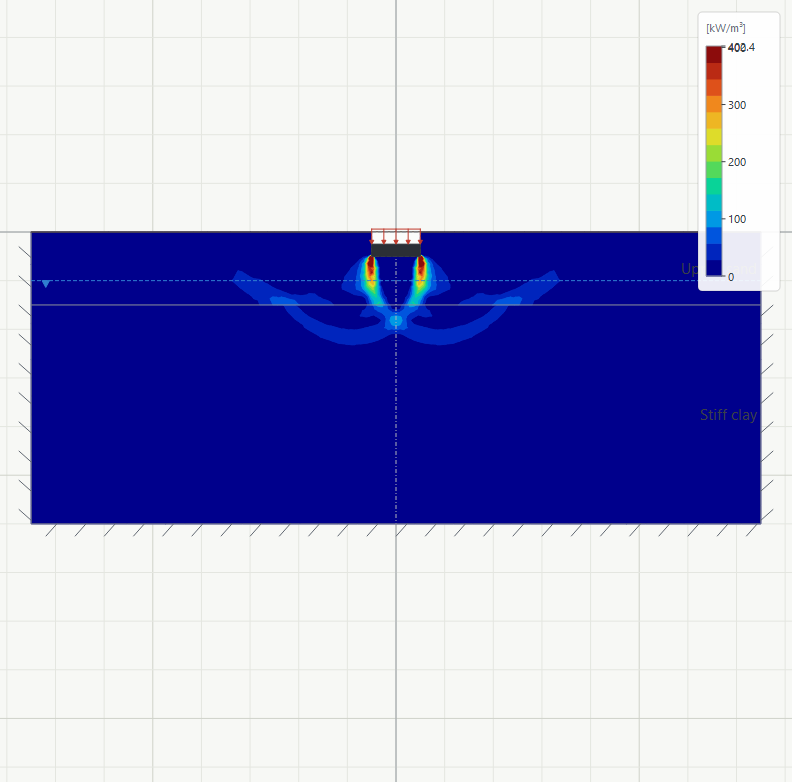
\includegraphics[width=0.48\textwidth]{output-failure-band}\hfill
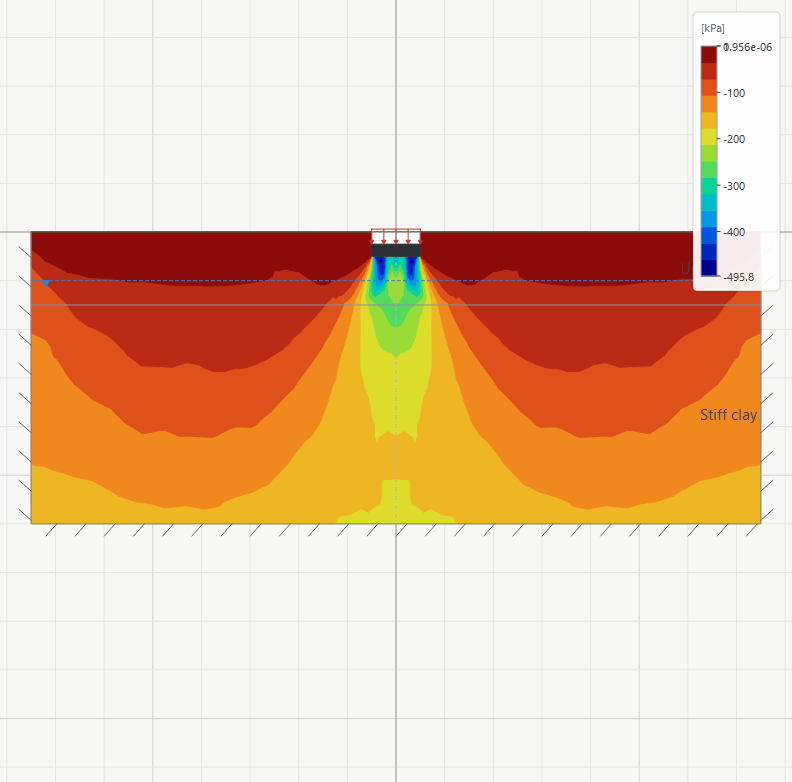
\includegraphics[width=0.48\textwidth]{output-vertical-stress}
\caption{Failure band (left) and vertical effective stress (right) for the demo model.}
\end{figure}

\subsection{Figure settings}
\field{Colour map} (\emph{rainbow} matches established FE packages; \emph{viridis} survives greyscale printing), \field{Contour bands}, \field{Rendering} (smoothed contours or exact element values for audit), \field{Value range} (automatic, full, or robust 1--99\,\% so a corner singularity cannot flatten the picture), \field{Section view} (mirrored full section or the analysed half), \field{Canvas grid} and the mesh and colour-scale overlays. None of these change the calculation.

\begin{tip}
The colour scale can be dragged anywhere on the canvas. Publication export (Section~\ref{sec:figures}) always uses a fixed legend gutter with the full field description.
\end{tip}

\subsection{Report figures}
\ui{Add current view to report} saves the view you are looking at --- colour map, bands, range, section view, grid and mesh overlay --- for the next report. \ui{Add finite-element mesh to report} adds a dedicated mesh figure. If nothing is saved, the report uses professional defaults: the mechanism, the failure band and the vertical stress.

% ================================================================== 11
\clearpage
\section{Failure envelope}\label{sec:envelope}

\begin{figure}[H]\centering
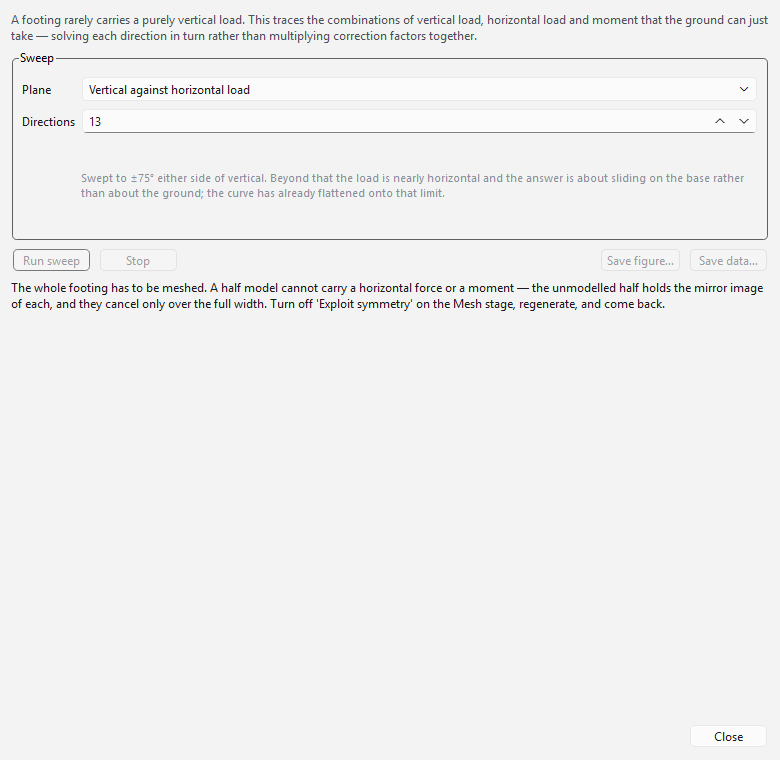
\includegraphics[width=0.8\textwidth,trim=0 300 0 0,clip]{dialog-envelope}
\caption{The failure-envelope tool before a sweep (the plot area below is filled once the sweep runs).}
\end{figure}

\menu{Analysis \textbar{} Failure envelope} (\key{Shift+F5}) sweeps the load direction and traces the combinations of vertical load, horizontal load ($V$--$H$ plane) or moment ($V$--$M$ plane) that the ground can just carry --- solving each direction in turn rather than multiplying correction factors together.

Choose the \field{Plane} and the number of \field{Directions} (each is a full pair of analyses), then \ui{Run sweep}. The result is a \emph{band}, not a curve: inside the green line is proved safe, outside the red line is proved to collapse, and the strip between is the numerical bracket. \ui{Save figure} writes an SVG; \ui{Save data} writes the swept points as CSV.

\begin{note}
The envelope needs the whole footing meshed: turn off \field{Exploit symmetry} on the Mesh stage first. The $V$--$H$ sweep stops at $\pm75^\circ$ from vertical (beyond that the question is base sliding); the $V$--$M$ sweep stops at $\pm40^\circ$ (beyond that the resultant leaves the footing).
\end{note}

% ================================================================== 12
\clearpage
\section{Independent capacity comparison}\label{sec:comparison}

\shot[0.9]{dialog-comparison}{The comparison view. The FELA interval is the shaded band; each classical method is placed relative to it.}

After every solve the software also evaluates the classical bearing-capacity methods (Terzaghi, Meyerhof, Brinch Hansen, Vesi\'c, Eurocode~7, AASHTO, IS~6403, BNBC, AIJ) and a method-of-characteristics solution, and places each against the FELA interval. Open it from \ui{View plot, tables and data} on the Output stage.

\begin{itemize}
  \item \ui{Overview} --- the chart. Green points fall inside the interval, red points outside, with the percentage from the nearest bound.
  \item \ui{All methods} --- the table: ultimate value, position, design value in each method's own safety format.
  \item \ui{Method details} --- one method at a time, with its breakdown, citation and warnings.
\end{itemize}

The status line states how comparable the methods are. \emph{Direct comparison} means the same idealisation. \emph{Indicative comparison --- layered idealisation} means the classical methods have taken the footing-base soil as a uniform half-space and cannot see the layers below; a large difference then usually means the FELA model is seeing something the formulas cannot, such as a weaker layer within the failure zone.

\begin{note}
The comparison is a cross-check, not a verification. Where a rigorous result and a code estimate disagree, the interpretation column says which assumption is responsible.
\end{note}

% ================================================================== 13
\clearpage
\section{Numerical verification study}\label{sec:study}

\shot[0.62]{dialog-verification}{Setting up an automatic study.}

\ui{Run verification study} on the Calculate or Output stage runs a sequence of trials on \emph{copies} of the project --- widening and deepening the domain, then refining the mesh --- until the result stops changing within the tolerance you set, or a declared limit is reached. The open model is never changed.

Choose a preset (\field{Quick}, \field{Engineering convergence}, \field{Research}) and, if you wish, the acceptance tolerances: change between trials, boundary-response limit and maximum bound gap. For a two-layer profile an optional upper-layer-thickness study can be added; it changes the physical model and is reported separately.

The results window gives a verdict (\emph{Converged --- recommended model} or the reason it is not), the recommended domain and mesh, the complete trial record, and publication-quality convergence plots. Everything can be exported as CSV, JSON, PNG or SVG, and the study is included in the report.

% ================================================================== 14
\clearpage
\section{Saving figures}\label{sec:figures}

\shot[0.72]{dialog-figure-export}{Publication figure export with live preview.}

\ui{Save figure} on the Output stage renders the current view off-screen at a chosen width (journal single column 90~mm, full width 180~mm, landscape 240~mm) as PNG (300 or 600~dpi), SVG or PDF. The crop can be the automatic model crop, the current view, or a rectangle you drag on the canvas. Options add the colour scale with the full field description, the mesh overlay, a coordinate grid, the title and a compact analysis footer. Settings are remembered between sessions.

% ================================================================== 15
\clearpage
\section{The calculation report}\label{sec:report}

\ui{Save report} on the Output stage writes the report as PDF (also HTML or plain text). It is structured as a calculation package a reviewer can sign:

\begin{enumerate}
  \item \textbf{Cover} --- document identity, the result card, the verification seal and a short model summary.
  \item \textbf{Model definition} --- the model as analysed (Figure~1), geometry and boundaries, the soil table, loading.
  \item \textbf{Method and assumptions} --- analysis settings, the design framework and its scope, and the numbered assumptions A1\ldots An made on your behalf.
  \item \textbf{Results} --- the summary table, the adaptive-refinement record and the result figures.
  \item \textbf{Verification and quality assurance} --- every admissibility check with its measured value against its limit, domain adequacy, the sensitivity study if run, and the solver status.
  \item \textbf{Independent capacity comparison} --- the chart and tables of Section~\ref{sec:comparison}.
  \item \textbf{References}.
  \item \textbf{Appendix A} --- the complete text record of the analysis, so that nothing in the body exists only in the summary.
\end{enumerate}

\begin{figure}[H]\centering
\fbox{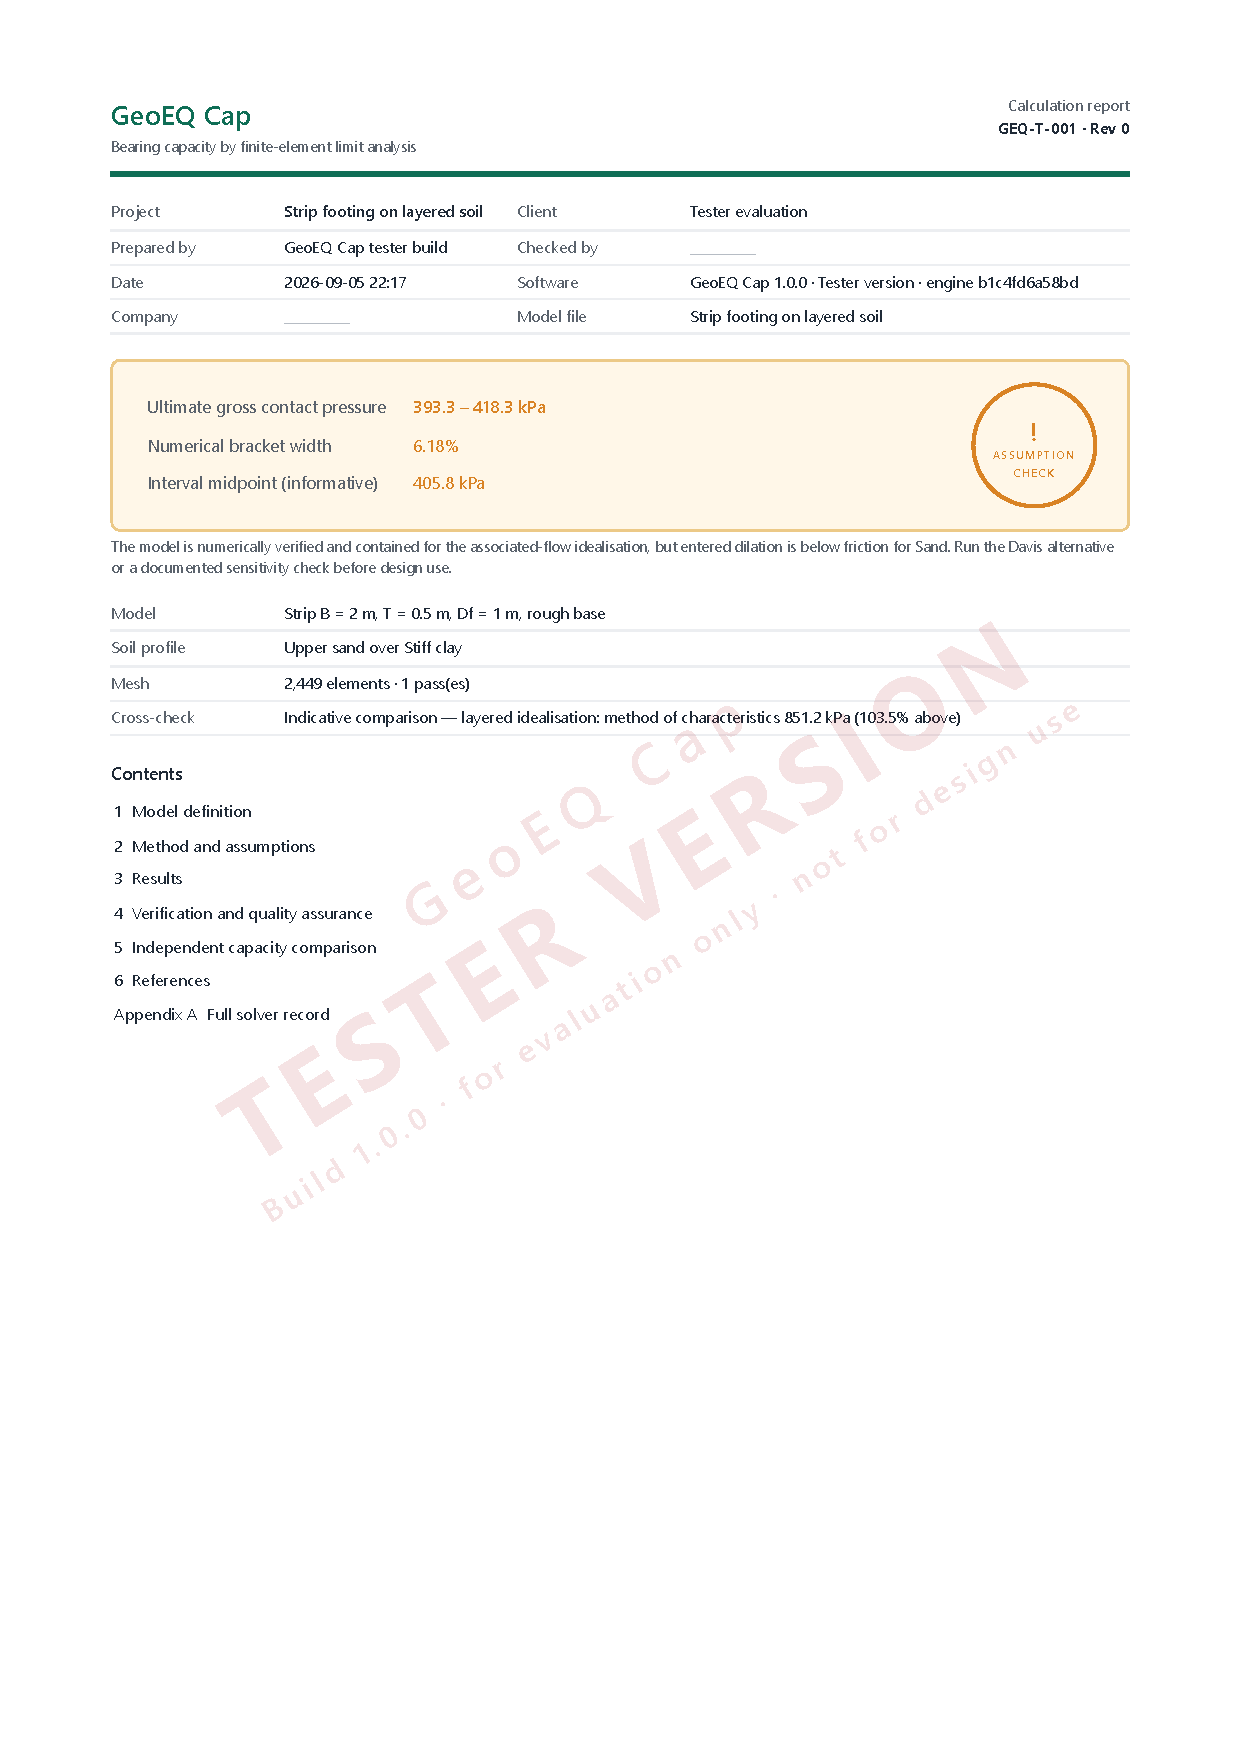
\includegraphics[width=0.45\textwidth,page=1]{tester-report.pdf}}\hfill
\fbox{\includegraphics[width=0.45\textwidth,page=5]{tester-report.pdf}}
\caption{Report cover (left) and the verification section (right), tester build.}
\end{figure}

\begin{tip}
Fill in the project identity (Section~\ref{sec:project}) before saving: the document number, revision and names go straight onto the cover, and a blank \field{Checked by} prints as a signing line.
\end{tip}

% ================================================================== 16
\clearpage
\section{Files, settings and updates}

\subsection{Project files}
Projects are saved as \texttt{.gec} files: a single readable text document containing the geometry, materials, layers, loads, mesh settings, analysis settings and project identity. The mesh and results are not stored; they are regenerated in seconds. Files are forward-compatible: a newer build opens older files, and an older build refuses a newer file with a clear message rather than misreading it.

\subsection{Application settings}
Figure-export preferences and dismissed notices are stored per user; they never travel with a project file.

\subsection{Privacy}
The application works fully offline. The only network access is the start-up update check, which downloads one small public file and sends nothing about you or your projects.

% ================================================================== 17
\section{Keyboard shortcuts}

\begin{tabularx}{\textwidth}{@{}lX@{}}
\toprule
\key{Ctrl+N} / \key{Ctrl+O} / \key{Ctrl+S} & New / Open / Save project\\
\key{Ctrl+P} & Project properties\\
\key{Ctrl+Z} / \key{Ctrl+Y} & Undo / Redo\\
\key{Ctrl+L} & Add soil layer\\
\key{Ctrl+M} & Material library\\
\key{F9} & Generate mesh\\
\key{Ctrl+Shift+M} & Show / hide mesh\\
\key{F5} & Calculate\\
\key{Shift+F5} & Failure envelope\\
\key{F} & Zoom to fit\\
\key{Ctrl++} / \key{Ctrl+-} & Zoom in / out\\
\key{Alt} while dragging & Override grid snap\\
\key{F1} & User manual\\
\bottomrule
\end{tabularx}

% ================================================================== 18
\section{Feedback}\label{sec:feedback}

As a tester, three things help most:

\begin{enumerate}
  \item \textbf{A case where the number surprised you.} Send the \texttt{.gec} file and say what you expected and why.
  \item \textbf{Anything unclear} in the interface or the report --- a label, a warning, a figure.
  \item \textbf{What is missing} for the work you actually do.
\end{enumerate}

Use \menu{Help \textbar{} Support and feature requests}, which opens the discussion board, or reply to the message that delivered this build.

% ================================================================== A
\appendix
\section{Verdicts and messages}\label{app:verdicts}

\subsection*{Result-card verdicts}
\begin{longtable}{L{34mm}L{120mm}}
\toprule
\textbf{Verdict} & \textbf{Meaning and action}\\
\midrule
\endhead
Verified model & Both bounds pass the independent admissibility checks and the mechanism is contained in the domain. The lower bound is a characteristic ultimate resistance; apply the selected design format before design use. No action.\\
Validated estimate & Circular footing: the near-bound interval passed the numerical and domain checks and is validated against exact circular benchmarks. No action; the report states that it is an estimate.\\
Assumption check & Numerically verified, but a material was entered with $\psi < \varphi$ while associated flow was used. Re-run with the Davis option or document a sensitivity check.\\
Check required & The collapse mechanism reaches a truncation boundary (or containment could not be checked). Widen or deepen the domain and re-run; the verification study does this automatically.\\
Not verified & At least one admissibility check failed. Do not use the values; review the model and re-run.\\
\bottomrule
\end{longtable}

\subsection*{Messages you may see}
\begin{longtable}{L{62mm}L{92mm}}
\toprule
\textbf{Message} & \textbf{Meaning}\\
\midrule
\endhead
The load is no longer symmetric, so the whole width is meshed automatically. & An inclined, eccentric, seismic or one-sided load is present. Nothing to do.\\
The mechanism comes close to the edge of the contour\ldots & The domain is probably adequate but a wider one would make sure. Consider widening.\\
Layer-interface slip detected. & The coloured interface is a real slip surface computed by the analysis.\\
Generate a mesh first. & Press \key{F9}.\\
The whole footing has to be meshed (envelope). & Turn off \field{Exploit symmetry} on the Mesh stage and regenerate.\\
Comparison unavailable & The classical methods cannot be evaluated for this case (for example seismic loading); the FELA result is unaffected.\\
This file was written by a newer version\ldots & Update the application from \menu{Help \textbar{} Check for updates}.\\
\bottomrule
\end{longtable}

\section{Glossary}
\begin{description}[style=nextline]
  \item[Lower bound] A load the ground can certainly carry, from a stress field in equilibrium that nowhere exceeds the strength.
  \item[Upper bound] A load at which collapse is certainly possible, from a kinematically admissible mechanism.
  \item[Bracket / relative gap] The interval between the two bounds, and its width relative to the mean.
  \item[Associated flow] The limit-analysis assumption $\psi = \varphi$.
  \item[Davis reduction] Conversion of $(c,\varphi,\psi)$ to an equivalent associated strength, giving a conservative result for $\psi < \varphi$.
  \item[Adaptive refinement] Repeated solve-and-refine passes that concentrate elements where the mechanism forms.
  \item[Truncation boundary] The artificial edge of the modelled ground; the mechanism must not reach it.
  \item[Characteristic resistance] The unfactored collapse resistance of the model; the design format factors it.
  \item[SRF] Strength-reduction factor: the factor by which $c$ and $\tan\varphi$ can be divided before a given pressure causes collapse.
  \item[Near bound] An axisymmetric result whose circumferential terms are enforced approximately; validated but not certified.
\end{description}

\vfill
\begin{center}\small\color{muted}
GeoEQ Cap User Guide, version 1.0 --- \href{https://github.com/geoeq/GeoEQ-Cap}{github.com/geoeq/GeoEQ-Cap}
\end{center}
\end{document}
